% Options for packages loaded elsewhere
\PassOptionsToPackage{unicode}{hyperref}
\PassOptionsToPackage{hyphens}{url}
%
\documentclass[
]{article}
\usepackage{lmodern}
\usepackage{amssymb,amsmath}
\usepackage{ifxetex,ifluatex}
\ifnum 0\ifxetex 1\fi\ifluatex 1\fi=0 % if pdftex
  \usepackage[T1]{fontenc}
  \usepackage[utf8]{inputenc}
  \usepackage{textcomp} % provide euro and other symbols
\else % if luatex or xetex
  \usepackage{unicode-math}
  \defaultfontfeatures{Scale=MatchLowercase}
  \defaultfontfeatures[\rmfamily]{Ligatures=TeX,Scale=1}
\fi
% Use upquote if available, for straight quotes in verbatim environments
\IfFileExists{upquote.sty}{\usepackage{upquote}}{}
\IfFileExists{microtype.sty}{% use microtype if available
  \usepackage[]{microtype}
  \UseMicrotypeSet[protrusion]{basicmath} % disable protrusion for tt fonts
}{}
\makeatletter
\@ifundefined{KOMAClassName}{% if non-KOMA class
  \IfFileExists{parskip.sty}{%
    \usepackage{parskip}
  }{% else
    \setlength{\parindent}{0pt}
    \setlength{\parskip}{6pt plus 2pt minus 1pt}}
}{% if KOMA class
  \KOMAoptions{parskip=half}}
\makeatother
\usepackage{xcolor}
\IfFileExists{xurl.sty}{\usepackage{xurl}}{} % add URL line breaks if available
\IfFileExists{bookmark.sty}{\usepackage{bookmark}}{\usepackage{hyperref}}
\hypersetup{
  hidelinks,
  pdfcreator={LaTeX via pandoc}}
\urlstyle{same} % disable monospaced font for URLs
\usepackage{longtable,booktabs}
% Correct order of tables after \paragraph or \subparagraph
\usepackage{etoolbox}
\makeatletter
\patchcmd\longtable{\par}{\if@noskipsec\mbox{}\fi\par}{}{}
\makeatother
% Allow footnotes in longtable head/foot
\IfFileExists{footnotehyper.sty}{\usepackage{footnotehyper}}{\usepackage{footnote}}
\makesavenoteenv{longtable}
\usepackage{graphicx,grffile}
\makeatletter
\def\maxwidth{\ifdim\Gin@nat@width>\linewidth\linewidth\else\Gin@nat@width\fi}
\def\maxheight{\ifdim\Gin@nat@height>\textheight\textheight\else\Gin@nat@height\fi}
\makeatother
% Scale images if necessary, so that they will not overflow the page
% margins by default, and it is still possible to overwrite the defaults
% using explicit options in \includegraphics[width, height, ...]{}
\setkeys{Gin}{width=\maxwidth,height=\maxheight,keepaspectratio}
% Set default figure placement to htbp
\makeatletter
\def\fps@figure{htbp}
\makeatother
\setlength{\emergencystretch}{3em} % prevent overfull lines
\providecommand{\tightlist}{%
  \setlength{\itemsep}{0pt}\setlength{\parskip}{0pt}}
\setcounter{secnumdepth}{-\maxdimen} % remove section numbering

\date{}

\begin{document}

\hypertarget{header-n2}{%
\section{Abstract Algebra Topic Summary}\label{header-n2}}

\begin{quote}
\emph{Abstract Algebra} TB: An Introduction to abstract algebra\_ by
Nicodemi, Sutherland and Towsley
\end{quote}

\textbf{Author:} \emph{Ryan G; 17805315}

Alternative/Accessible Textbooks:

\begin{itemize}
\item
  \href{http://booksdescr.org/item/index.php?md5=8116F6EE260EE2681415ABFD600696AC}{\emph{An
  Introduction to Abstract Algebra} by Derek Robinson}
\item
  \href{http://booksdescr.org/item/index.php?md5=7519238B77AC24ABEEB6B3F4A0A1392F}{\emph{Abstract
  Algebra: An Introduction} by Thomas Hungerford}
\item
  \href{http://booksdescr.org/item/index.php?md5=D4CCAD47CC508CFE7C7DD857AB0AEF98}{\emph{Introduction
  to Modern Abstract Algebra} by David Burton}
\end{itemize}

\tableofcontents

\begin{center}\rule{0.5\linewidth}{\linethickness}\end{center}

\hypertarget{header-n17}{%
\section{1) Induction and Divisibility}\label{header-n17}}

\begin{quote}
\textbf{\emph{Week 1 Material, Due Thur. 7 March TB: {[}1.1{]},
{[}1.2{]}, {[}2.1{]}, {[}2.2{]} }}
\end{quote}

\begin{itemize}
\item
  \protect\hyperlink{aaux281ux29sets}{Numbers and Sets}
\end{itemize}

\hypertarget{header-n26}{%
\subsection{Numbers and Sets}\label{header-n26}}

This is mostly reproduced in the Topic 1 section on Sets in the
\href{https://ryangreenup.github.io/AnalysisNotes/AnalysisNotes.html\#an(1)sets}{Analysis
Notes}

\hypertarget{header-n28}{%
\subsubsection{Set Orders}\label{header-n28}}

The Natural Numbers have an intuitive order:

\(0<1<2<3<4 \dots\)

As to the Real Numbers:

\(-99<-1<0<e<\pi<e^{4\pi}<\frac{999}{2}\)

However, the \protect\hyperlink{aaux285ux29rings2}{Field of Complex
Numbers} has no intuitive order because the numbers do not exist on a
line but on a plane.

On a line mathematical operations can be seen as a symmetrical
transformation of that line, but on a plane order becomes somewhat
arbitrary.
\href{https://www.youtube.com/watch?v=mvmuCPvRoWQ}{*3Blue1Brown} has a
great video on this.

\hypertarget{header-n35}{%
\subsubsection{Mathematical Induction}\label{header-n35}}

Refer to
\href{https://ryangreenup.github.io/AnalysisNotes/AnalysisNotes.html\#an(1)wop}{these
notes} in Analysis, they overlap entirely.

\hypertarget{header-n37}{%
\subsection{Arithmetic and Divisibility}\label{header-n37}}

Whats important here, is the division Algorithm, which states:

\begin{quote}
If an integer is divided by some \(b \in \mathbb{N} \) , there will
always be some remainder \(r \enspace : \enspace 0<r<b\)
\end{quote}

This is a pretty straightforward proposition, but it underlies all later
proofs of abstract algebra.

\hypertarget{header-n43}{%
\subsubsection{Properties of the Integers}\label{header-n43}}

Investigating the properties of number sets will be important later for
considering the algebraic structure of sets, but for now, consider the 6
properties of the integers:

\begin{enumerate}
\def\labelenumi{\arabic{enumi}.}
\item
  \textbf{Associative} under addition and multiplication

  \begin{enumerate}
  \def\labelenumii{\arabic{enumii}.}
  \item
    \(\forall (a,b,c \in \mathbb{Z}), a + (b+c) = (a+b) + c\)
  \item
    \(\forall (a,b,c \in \mathbb{Z}), a \cdot (b\cdot c) = (a\cdot b) + c\)
  \end{enumerate}
\item
  \textbf{Commutative} under multiplication and addition

  \begin{enumerate}
  \def\labelenumii{\arabic{enumii}.}
  \item
    \(\forall (a,b \in \mathbb{Z}),  a + b = b + a\)
  \item
    \(\forall (a,b \in \mathbb{Z}),  a \cdot b = b \cdot a\)
  \end{enumerate}
\item
  There always exists a unique \textbf{additive Identity}, \(0\)

  \begin{enumerate}
  \def\labelenumii{\arabic{enumii}.}
  \item
    \(\forall x \in \mathbb{z}, !\exists 0 : 0+x=x\)
  \end{enumerate}
\item
  There always exists a unique \textbf{multiplicative identity}, \(1\)

  \begin{enumerate}
  \def\labelenumii{\arabic{enumii}.}
  \item
    \(\forall x \in \mathbb{z}, !\exists 1 : 1\cdot x=x\)
  \end{enumerate}
\item
  Every integer has an \textbf{additive inverse}\textbackslash{}

  \begin{enumerate}
  \def\labelenumii{\arabic{enumii}.}
  \item
    \(\forall x \in \mathbb{Z}, \exists (-x) : x + (-x) = 0\)
  \end{enumerate}
\item
  Addition and multiplication satisfy the \textbf{distributive law}

  \begin{enumerate}
  \def\labelenumii{\arabic{enumii}.}
  \item
    \(\forall (x,y,z \in \mathbb{Z}), (x\cdot y) + (x\cdot z)\)
  \end{enumerate}
\end{enumerate}

\hypertarget{header-n80}{%
\subsubsection{Divisibility Definition}\label{header-n80}}

Let \(a\) and \(b\) be integers with \(b \neq 0\):

\[(a,b) \in \mathbb{Z} : b \neq 0\]

it is said that \(b\) \textbf{divides} \(a\) (written \(b|a\)), if there
is some integer \(q\) such that \(\enspace a = b\cdot q\):

\[b|a \iff \exists q \in \mathbb{Z} : a = b\cdot q\]

This is the same as saying:

\begin{itemize}
\item
  \(a\) is \textbf{divisible} by \(b\)
\item
  \(a\) is a \textbf{multiple} of \(b\)
\end{itemize}

\hypertarget{header-n91}{%
\subsubsection{Divisibility Properties}\label{header-n91}}

\begin{enumerate}
\def\labelenumi{\arabic{enumi}.}
\item
  \(a|b \enspace  \wedge \enspace b|c \implies a|c\)
\item
  \(a|b \enspace \wedge \enspace a|c \implies a|(mb + nc)\)
\end{enumerate}

\#\#\#\#

\hypertarget{header-n98}{%
\subparagraph{Proof}\label{header-n98}}

Observe that:\\
\(a|b \implies b = k\cdot a, \enspace \exists t \in \mathbb{Z} \quad \text{and} \quad b|c \implies c = s \cdot b, \enspace \exists s \in \mathbb{z}\)

\hypertarget{header-n100}{%
\subsubsection{Division Algorithm}\label{header-n100}}

The definition of the algorithm:

Let \(a\) and \(b\) bey any integers with \(b >0\).

There are unique integers \(q\) and \(r\) such that \(a = qb +r\), where
\(0 \leq r <b\), i.e.:

\[!\exists (q,r \in \mathbb{Z}, \enspace q \neq r)  : (a = qb +r) \wedge (0 \leq r < b)\]

\hypertarget{header-n105}{%
\subsection{Greatest Common Divisors and Euclids
Algorithm}\label{header-n105}}

\hypertarget{header-n106}{%
\subsubsection{Definition of the GCD}\label{header-n106}}

Suppose \(a\) and \(b\) are nonzero integers, the \emph{greatest common
divisor} of \(a\) and \(b\) is the largest integer that divides both of
them and is denoted:

\(gcd(a,b)\)

Observe some properties of the gcd

\begin{enumerate}
\def\labelenumi{\arabic{enumi}.}
\item
  \(\gcd(0,0)\) is undefined because it would be 
\item
  \(\gcd(a,0) = a\) ; because any number divides and the largest number
  that divides is itself

  \begin{enumerate}
  \def\labelenumii{\arabic{enumii}.}
  \item
    unless \(a=0\) in which case it would be like (1) above.
  \end{enumerate}
\item
  \(\gcd(b, qb) = b\) ; because the \(b\) divides both terms and is the
  largest possible divisor of\(b\)
\end{enumerate}

\hypertarget{header-n120}{%
\subsubsection{Theorem 1}\label{header-n120}}

The \(\gcd(a,b)\) is the smallest positive integer that can be expressed
in the form:

\[ma + nb : (m,n \in \mathbb{Z})\]

\hypertarget{header-n123}{%
\paragraph{Corollary}\label{header-n123}}

Observe further, that for \(x \in \mathbb{Z}\) , thwse two statements
are wholly equivalent:

\begin{enumerate}
\def\labelenumi{\arabic{enumi}.}
\item
  \(x = ma+nb\)
\item
  \$\textbackslash gcd(a,b)\textbar x
\end{enumerate}

\begin{quote}
i.e. \(x = ma + nb \iff \gcd(a,b) | x\)
\end{quote}

\hypertarget{header-n133}{%
\subsubsection{Relatively Prime}\label{header-n133}}

\hypertarget{header-n134}{%
\paragraph{Definition}\label{header-n134}}

Suppose \(a\) and \(b\) are non-zero integers, they are \emph{relatively
prime} (i.e. \emph{coprime}) if \(\gcd(a,b)=1\)

\hypertarget{header-n136}{%
\paragraph{Proposition; Relatively Prime by GCD}\label{header-n136}}

Suppose \(a\) and \(b\) are non-zero integers, and let \(\gcd(a,b) =d\)

Then \(\frac{a}{d}\) and \(\frac{b}{d}\) are relatively prime.

\hypertarget{header-n139}{%
\subsubsection{Euclid's Lemma (P.18)}\label{header-n139}}

\hypertarget{header-n140}{%
\paragraph{Definition}\label{header-n140}}

Suppose \(a, b, c\) are integers such that \(a\) and \(b\) are coprime.

if \(b\cdot c\) is a multiple of \(a\),

Then \(c\) must be a multiple of \(a\)

(because \(p\) was prime)

\hypertarget{header-n145}{%
\subsubsection{Theorem; GCD becomes Remainder and
Factor}\label{header-n145}}

Suppose \((a,b,q,r)\) are all integers, such tat:

\[a = qb +r\]

Then,

\[\gcd(a,b) =\gcd(b,r)\]

\hypertarget{header-n150}{%
\subsubsection{Euclid's Algorithm (i.e. Calculating
GCD's)}\label{header-n150}}

\emph{Euclid's Algorithm} allows for a method to find the \emph{Greatest
Common Denominator}:

For two positive natural numbers, \(a,b\) such that \(a>b\):

\begin{enumerate}
\def\labelenumi{\arabic{enumi}.}
\item
  write in the form of \(a=qb+r\), where \((q,r\in \mathbb{Z})\) with
  \(0<r<b\)
\item
  If \(r=0\), then \(a=q\cdot b\) and hence \(\gcd(a,b) = \gcd(b,r)\)
\item
  if \(r\neq\) 0, then \(\gcd(a,b) = \gcd(b,r)\)

  \begin{enumerate}
  \def\labelenumii{\arabic{enumii}.}
  \item
    Now repeat from step 1 
  \end{enumerate}
\end{enumerate}

\hypertarget{header-n163}{%
\subsubsection{Lowest Common Multiples}\label{header-n163}}

For two integers \((a,b) \in \mathbb{Z}\), the \emph{Lowest Common
Multiple}, is the smallest integer that is a multiple of both \(a\) and
\(b\)

The \(LCM\) is a number that is the smallest possible multiple of other
numbers

\hypertarget{header-n166}{%
\paragraph{\texorpdfstring{Finding the
\emph{LCM}}{Finding the LCM}}\label{header-n166}}

In order to find the \emph{LCM} use the formula:

\[\text{lcm} (a,b) = \frac{a\cdot b}{\gcd(a,b)}\]

\begin{center}\rule{0.5\linewidth}{\linethickness}\end{center}

\hypertarget{header-n170}{%
\section{(2) Prime Numbers}\label{header-n170}}

\protect\hyperlink{antoc}{Back to Top}

\hypertarget{header-n173}{%
\subsection{Definitions}\label{header-n173}}

Prime and composite numbers are any numbers that satisfy the following
conditions:

\begin{longtable}[]{@{}ll@{}}
\toprule
Prime Numbers & Composite Numbers\tabularnewline
\midrule
\endhead
\( 1. \enspace p>1 \\ 2. \enspace p \in \mathbb{z} \\ 3. \enspace  x|p \iff (x =1 \enspace \wedge \enspace x=p)\)
&
\(1. \enspace c > 1 \\ 2. \enspace c \text{ is not prime}\)\tabularnewline
\bottomrule
\end{longtable}

Observe that \(1\) is neither a prime nor a composite number, this is
important for later

\hypertarget{header-n183}{%
\subsection{Infinite Primes}\label{header-n183}}

\hypertarget{header-n184}{%
\subsubsection{Summary}\label{header-n184}}

There are infinite prime numbers

\hypertarget{header-n186}{%
\subsubsection{Proof}\label{header-n186}}

Suppose;

\[S = \{p_1, p_2, p_3, \dots p_n\}\]

is the set of the first \(n\) prime numbers,

let:

\[q = (p_1 \cdot p_2 \cdot p_3 \cdot \dots p_n)\]

Observe that \(q\) would not be a multiple of any value \(p \in S\)

\begin{quote}
Although this does not mean \(q\) is necessarily prime (primes can be
\href{https://www.youtube.com/watch?v=tlpYjrbujG0}{much more difficult}
to generate), \(q\) is possible a composite of primes not in \(S\), but
regardless, \(q\) is not divisible by any \(p \in S\)
\end{quote}

Thus \(S\) cannot contain all prime values.

Observe likewise, no set \(S\) could be constructed such that it
contained all the primes

\begin{quote}
or atleast no finite set \(S\)
\end{quote}

\(\therefore\) , the set of all Prime numbers must not be finite (i.e.
there are infinite primes).

\hypertarget{header-n202}{%
\subsection{Primes of Multiples}\label{header-n202}}

If a prime number divides a composite, it must divide one of\\
the factors of that composite number

\hypertarget{header-n204}{%
\subsubsection{Summary}\label{header-n204}}

\(p\) is a prime number \emph{if and only if}:

\[\forall (a,b \in \mathbb{z}), \enspace p|a\cdot b \implies p|a \enspace \vee \enspace p|b\]

\hypertarget{header-n207}{%
\subsubsection{Proof}\label{header-n207}}

Suppose \(p\) is a prime number:

\[\enspace p | (a \cdot b)\]

Either \(p\) divides \(a\) or it does not:

\begin{longtable}[]{@{}ll@{}}
\toprule
\(p\mid a\) & \(p\nmid a\)\tabularnewline
\midrule
\endhead
\(p\mid a\) , thus\textless br
/\textgreater{}\(p\mid ab \implies p|a \vee p|b \quad \blacksquare\) &
\(p \nmid a\), thus:\textless br /\textgreater{}\textless br
/\textgreater{}\(gcd(a,p) = 1\) \textless br /\textgreater{}\textless br
/\textgreater{} because \(p|ab\) and \(\gcd(a,p) = 1\)\textless br
/\textgreater{}\textless br /\textgreater{}Then by Euclid's
Lemma:\textless br /\textgreater{}\(p|b\)\textless br
/\textgreater{}\textless br /\textgreater{}thus, \textless br
/\textgreater{}\(p|ab \implies p|a \vee p|b \quad \blacksquare\)\tabularnewline
\bottomrule
\end{longtable}

Thus:

\[p|ab \implies p|a \vee p|b\]

\hypertarget{header-n220}{%
\subsection{Prime Factors}\label{header-n220}}

\hypertarget{header-n221}{%
\subsubsection{Summary}\label{header-n221}}

Suppose \(p\) is prime and \(p\) divides some number
\(a_1 \cdot a_2 \cdot a_3 \dots a_n\)

Then \(p\) divides \(a_k \enspace : \enspace 1 \leq k \leq n\)

Moreover, if \(a_k\) is prime, then \(p=a_k\)

\hypertarget{header-n225}{%
\subsection{The Fundamental Theorem of Arithmetic}\label{header-n225}}

\hypertarget{header-n226}{%
\subsubsection{Summary}\label{header-n226}}

For any integer \(n\):

\begin{enumerate}
\def\labelenumi{\arabic{enumi}.}
\item
  \(\enspace n = p^{k_1}_1\cdot p^{k_2}_2 \cdot p^{k_3}_3 \dots p^{k_m}_m\)
\item
  The above factorisation of \(n\) is unique to the value of \(n\)
\end{enumerate}

This proof is provided on p. 28 of the TB.

\hypertarget{header-n234}{%
\subsubsection{Corollary, Rational Numbers}\label{header-n234}}

Every rational number can be expressed in a lowes form of relatively
prime integers.

\hypertarget{header-n236}{%
\paragraph{Summary}\label{header-n236}}

Every rational number can be expressed uniquely as some fraction of
integers:

\[\forall r \in \mathbb{Q}, \enspace !\exists m,n \in \mathbb{Z} : r = \frac{m}{n}\]

\hypertarget{header-n239}{%
\subparagraph{\texorpdfstring{\(\sqrt{2}\) is not
rational}{\textbackslash sqrt\{2\} is not rational}}\label{header-n239}}

A rational number can be expressed as a ratio, \(\sqrt{2}\) cannot be,
the proof is in the
\href{http://booksdl.org/get.php?md5=ef3626243a81006414e1f5a67ce694e0}{Analysis
Textbook} at {[}2.1.4{]}.

Proof

Just refer to the textbook

\hypertarget{header-n243}{%
\subsection{Theorems of Euler and Fermat (ch.
{[}1.7{]})}\label{header-n243}}

\hypertarget{header-n245}{%
\subsubsection{Euler-Phi Function}\label{header-n245}}

The \emph{Euler-Phi Function} counts the number of integers relatively
prime to \(n\) that are less than \(n\),

\hypertarget{header-n247}{%
\paragraph{Definition}\label{header-n247}}

for \(n \geq 1\);

\(\phi(n)\) is the number of positive integers less than or equal to
\(n\) that are relatively prime to \(n\)

\begin{quote}
e.g. \(2, 3, 7\) are relatively prime to \(10\), thus \(\phi(10) = 3\)
\end{quote}

\hypertarget{header-n252}{%
\subsubsection{Powers of Euler-Phi Function}\label{header-n252}}

\hypertarget{header-n253}{%
\paragraph{Summary}\label{header-n253}}

if \(p\) is prime and \(i \geq 1\),

\begin{align}
\phi(p^i) &= p^i - p^{i-1} \\
&=p^i(1-frac{1}{p})
\end{align}

\hypertarget{header-n256}{%
\paragraph{Proof}\label{header-n256}}

All the numbers between \(1\) and \(p-1\) are relatively prime to p,
thus \(\phi(p)=p-1\).

All integers less than \(p^i\) (for \(i\geq 1\)) are relatively prime to
\(p^i\) except for multiples of \(p\).\\
i.e. all values less than \(p^i\) are relatively prime except for
\(1p,2p,3p \dots p^(i-1) p\).

So there are exactly \(p^{i-1}\) multiples of \(p\) that are multiples
and hence not relatively prime.

Thus there is a total of \(p^i-p^{i-1}\) numbers between \(1\) and
\(p^i\) that are relatively prime to \(p^i\).

\hypertarget{header-n261}{%
\subsubsection{Euler-Phi Function is Multiplicative}\label{header-n261}}

\hypertarget{header-n262}{%
\paragraph{Summary}\label{header-n262}}

For positive relatively prime integers \(m\) and \(n\):

\[\gcd(m, n) = 1 \implies \phi(m \cdot n) = \phi(m) \cdot \phi(n)\]

\hypertarget{header-n265}{%
\paragraph{Proof}\label{header-n265}}

Refer to p. 44 of the TB.

\hypertarget{header-n267}{%
\paragraph{Corollary}\label{header-n267}}

for primes \(p, e \in \mathbb{N}\),

Given some \(n\) value:

\[n = p^{e_1}_1 \times p^{e_2}_2 \times p^{e_3}_3 \times p^{e_r}_r\]

Then the Euler Phi function is:

\[\phi(n) = p^{e_1-1}_1 \cdot (p_1-1) \times p^{e_2-1}_2 \cdot (p_2-1) \times p^{e_3-1}_3 \cdot (p_3-1) \dots p^{e_r-1}_r \cdot (p_r-1)\]

Further it follows:

\[\phi(n) = n \times \frac{p_1 -1}{p_1} \times \frac{p_2 -1}{p_2} \times \frac{p_3 -1}{p_3} \times \frac{p_r -1}{p_r}\]

\begin{quote}
I've merely interchanged \(\cdot\) and \(\times\) here\\
for want of illustration, there is no significant\\
meaning right here whatsoever (where as maybe\\
later down \(\cdot\) may refer to more abstract\\
ideas of multiplication but it's pretty lose as it stands)
\end{quote}

\hypertarget{header-n278}{%
\subsubsection{Eulers Theorem}\label{header-n278}}

\hypertarget{header-n280}{%
\paragraph{Summary}\label{header-n280}}

For relatively prime integers \(a\) and \(m \geq 1\):

\[m | (a^{\phi(m)} - 1)\]

\hypertarget{header-n283}{%
\paragraph{Proof}\label{header-n283}}

The proof is on page 45 of the TB.

\hypertarget{header-n285}{%
\paragraph{Fermats Little Theorem}\label{header-n285}}

The special case of \emph{Euler's Theorem}, men \(m\) is prime, in known
as \emph{Fermat's Little Theorem}.

\hypertarget{header-n287}{%
\subparagraph{Summary}\label{header-n287}}

For some prime \(p\) and integer \(a\):

\[p \mid (a^p -a)\]

\hypertarget{header-n290}{%
\subparagraph{Proof}\label{header-n290}}

It must be such that \(p\) divides \(a\) or \(p\) does not divide \(a\)
, hence:

\begin{longtable}[]{@{}ll@{}}
\toprule
\(p \mid a\) & \( p \nmid a\)\tabularnewline
\midrule
\endhead
if \(p \mid a\) \textless br
/\textgreater{}\(\implies p \mid a^n, \enspace \exists n \in \mathbb{N}\)\textless br
/\textgreater{} \(\implies p \mid a^{p-1}\) \textless br /\textgreater{}
\(\implies p \mid (a^p -a)\) & if \(p\nmid a\)\textless br
/\textgreater{}\textless br /\textgreater{}Then \(p\) and \(a\) are
relatively prime, thus, \emph{Eulers Theorem} applies;\textless br
/\textgreater{}\textless br /\textgreater{}By \emph{Euler's
Theorem}:\textless br /\textgreater{}\(p|(a^{\phi(p)}-1)\)\textless br
/\textgreater{}\(\implies p \mid (a^{(p^1-p^0)}-1)\)\textless br
/\textgreater{}\(\implies p \mid (a^{(p-1)}-1)\)\textless br
/\textgreater{}\(\implies p \mid (a \cdot (a^{(p-1)}-1))\)\textless br
/\textgreater{}\(\implies p \mid (a^p-a)\)\tabularnewline
\bottomrule
\end{longtable}

Thus for a prime \(p\) and integer \(a\):

\[p \mid (a^p - a)\]

\begin{center}\rule{0.5\linewidth}{\linethickness}\end{center}

\hypertarget{header-n302}{%
\section{(3) Relations and Congruence}\label{header-n302}}

\protect\hyperlink{antoc}{Back to Top}

\begin{itemize}
\item
  \protect\hyperlink{aaux283ux29rel}{Relations}
\item
  \protect\hyperlink{aaux283ux29con}{Congruence Modulo n}
\item
  \protect\hyperlink{aaux283ux29ringintro}{The Ring}
\end{itemize}

\hypertarget{header-n312}{%
\subsection{Relations}\label{header-n312}}

A relation on a set \(A\) is a subset \(R\) of the cartesian product:

\[A\times A = \{(a,b) : a,b \in A\}\]

if \((a,b) \in R\) we write that \(\enspace a \enspace R \enspace b\)

\hypertarget{header-n317}{%
\subsubsection{Example}\label{header-n317}}

If we had the relation \(<\) on the set \(A\) = \{1,2,3\}.

The Cartesian product would be:

\[A \times A = \{(1,1), (1,2), (1,3), (2,1), (2,2), (2, 3), (3, 1), (3, 2), (3,3)\}\]

The set corresponding to the relation \(<\) would be:

\[\{(1,2), (1, 3), (2, 3)\}\]

\hypertarget{header-n323}{%
\subsubsection{Relation Types}\label{header-n323}}

\begin{itemize}
\item
  \textbf{Reflexive} relations are relations where

  \begin{itemize}
  \item
    \(a \enspace R \enspace a\)

    \begin{itemize}
    \item
      \(\forall a \enspace \in A\)
    \end{itemize}
  \end{itemize}
\item
  \textbf{Symmetric} relations are such that

  \begin{itemize}
  \item
    \(a \enspace R \enspace b \implies b \enspace R \enspace a\)

    \begin{itemize}
    \item
      \(\forall a, b \in A\)
    \end{itemize}
  \end{itemize}
\item
  \textbf{Transitive} relations are such that

  \begin{itemize}
  \item
    \(a \enspace R \enspace b \quad \wedge \quad  b \enspace R \enspace c \implies  b \enspace R \enspace a\)

    \begin{itemize}
    \item
      \(\forall a,b,c\in A\)
    \end{itemize}
  \end{itemize}
\end{itemize}

An equivalence relation is a relation that is reflexive, symmetric and
transitive.

\hypertarget{header-n350}{%
\paragraph{Example 1}\label{header-n350}}

Let \(S = \{\text{all people}\}\)

We will define a relation \(R\) as satisfied if thouse people share the
same parents

\hypertarget{header-n353}{%
\subparagraph{Define a relation}\label{header-n353}}

\(x \enspace R \enspace y\) if \(x\) has the same parents as \(y\)

observe the following properties:

\begin{itemize}
\item
  \textbf{Reflexivity}; any person will be related to themselves because
  they share the same parents
\item
  \textbf{symmetry}; If percy is related to Fred, then they share
  parents and hence then Fred must be related to Percy.
\item
  \textbf{Transivity}; If Percy is related to Fred and Fred is Related
  to Ron, Ron and Percy must share parents, thus Ron and Percy are
  Related.
\end{itemize}

\hypertarget{header-n363}{%
\paragraph{Example 2}\label{header-n363}}

Let \(S\) be all real numbers

\hypertarget{header-n365}{%
\subparagraph{Define a Relation:}\label{header-n365}}

\(x<y \iff x \enspace R \enspace y\)

observe the following properties:

\begin{itemize}
\item
  \textbf{Non-Reflexive}; any number is not less than its own value.
\item
  \textbf{Non-Symmetry}

  \begin{itemize}
  \item
    Take 5 and 7, if \(5<7\) , then \(7 \nless 5\)
  \end{itemize}
\item
  \textbf{Transitive}; It is true that if, say, \(3<4\) and \(4<5\) then
  \(3<5\)

  \begin{itemize}
  \item
    This property is why we ordinarily write interval notation in this
    format, e.g. \(x\in (3,5) \iff 3<x<5\)

    \begin{itemize}
    \item
      Be careful though, using greater than symbols is not transitive
      per se and may lead to making transcription errors.
    \end{itemize}
  \end{itemize}
\end{itemize}

\hypertarget{header-n384}{%
\subsubsection{Equivalence Class }\label{header-n384}}

Given a relation \(R\) on some set \(A\),

If \([a]\) is the set of all elements of \(A\) that satisfy the relation
for \(a\):

\[[a]_R = [a] = \{b \in A : b\enspace R \enspace a\}\]

This is called the \emph{equivalence class of} \(a\) \emph{with respect
to} \(R\)

\hypertarget{header-n389}{%
\paragraph{Example}\label{header-n389}}

Let \(S\) all real numbers.

\textbf{Define a relation:}

\(x \enspace R \enspace y \iff x < y\)

Let's find the equivalence class of \([6]\):

\([6]_R = \{1,2,3,4,5\}\)

\hypertarget{header-n395}{%
\paragraph{Proposition}\label{header-n395}}

Let \(R\) be an equivalence relation on \(A\):

if \(a,b \in A\), then either,

\begin{itemize}
\item
  \([a] = [b]\), OR
\item
  \([a]\cap [b] = \emptyset\)
\end{itemize}

So if \(a\) and \(b\) are both elements of \(A\), then their equivalence
classes are identical or absolutely different.

\hypertarget{header-n405}{%
\subsection{\texorpdfstring{Congruence Modulo
\emph{n}}{Congruence Modulo n}}\label{header-n405}}

Let \(a, b \in \mathbb{Z}\) and \(n \in \mathbb{Z}^{+}\)

We say that:

\(a\) and \(b\) are *congruent modulo n\( if \)n \textbackslash mid
(a-b)\$, and it is expressed:

\[a\equiv b \enspace \pmod{n}\]

or in other words:

\[a\equiv b \enspace (mod n) \iff a = b + q\cdot n : q \in \mathbb{R}\]

\hypertarget{header-n414}{%
\subsubsection{Further Notation;}\label{header-n414}}

Generally the notation:

\[a \mod n = r\]

Refers to the remainder after \(a\) has been divided by \(n\) (i.e. the
residue of \(a\) modulo \(n\))

So be careful:

\begin{longtable}[]{@{}ll@{}}
\toprule
\textbf{This is a number} & \textbf{This is a statement about
Divisibility}\tabularnewline
\midrule
\endhead
\(a \mod n = r\) & \(a\equiv b \enspace \pmod{n}\)\tabularnewline
\bottomrule
\end{longtable}

\hypertarget{header-n426}{%
\subsubsection{The Euclidean Algorithm}\label{header-n426}}

if \(a = q\cdot b +r\) then \(a\equiv b \enspace \pmod{n}\)

Recall from the \emph{Euclidean Algorithm}:

\[a = q\cdot b +r \implies \gcd(a,b) = \gcd(b,r)\]

This translates to:

\(a \equiv r \pmod{b} \implies \gcd(a,b) = \gcd(b,r)\)

\hypertarget{header-n432}{%
\paragraph{Eulers Theorem}\label{header-n432}}

\emph{Euler's Theorem} (and hence *Fermat's Little Theorem) can now be
restated in terms of modulos.

For relatively prime integers \(a\) and \(m \geq 1\):

\begin{align}
m \mid (&a^{\phi (m)}-1) \\
&a^{\phi (m)} \equiv 1 \pmod{m}
\end{align}

\hypertarget{header-n436}{%
\subparagraph{Fermats Little Theorem}\label{header-n436}}

The special case of \(Euler's Theorem\), when \(m\) is prime, is known
as \emph{Fermat's Little Theorem}.

\[p \mid (a^p-a) \\
a^p \equiv a \pmod{p}\]

\hypertarget{header-n439}{%
\subsubsection{\texorpdfstring{Residue of \(a\) modulo \(n\) (i.e.
remainder of Division
Algorithm)}{Residue of a modulo n (i.e. remainder of Division Algorithm)}}\label{header-n439}}

If \(a,b \in \mathbb{Z}\) and \(n \in \mathbb{Z}^+\)

Then \(a = b \pmod{n}\) if and only if \(a\) and \(b\) have the same
remainder when divided by \(n\).

If the remainder is \(r\) then:

\[a \equiv r \pmod{n}\]

\begin{quote}
i.e. \(a = p\cdot n +r, \enspace \exists p \in \mathbb{R}\)
\end{quote}

This valur \(r\) is known as the *residue of a modulo n\$ and can always
be found to exist.

\hypertarget{header-n447}{%
\subsubsection{Mod Laws}\label{header-n447}}

Let \(n \in \mathbb{Z}^+\) and \( a,b,c,d, k \in \mathbb{Z}
nd \)m \textbackslash in \textbackslash mathbb\{N\}\$

\begin{enumerate}
\def\labelenumi{\arabic{enumi}.}
\item
  \(a \equiv b \pmod{n} \implies k\cdot a \equiv k\cdot b \pmod{n}\)
\item
  \(\Big( a \equiv b \pmod{n} \enspace \wedge \enspace c = d \pmod{n} \Big)\)

  \begin{enumerate}
  \def\labelenumii{\arabic{enumii}.}
  \item
    \(\implies (a+c) \equiv (b+d) \pmod{n}\), and also
  \item
    \(\implies (a\cdot c) \equiv (b\cdot d) \pmod{n}\)
  \end{enumerate}
\end{enumerate}

\hypertarget{header-n459}{%
\subsubsection{Congruence Class}\label{header-n459}}

Let \(n \in \mathbb{Z}^+\) and \(a \in \mathbb{Z}\)

The congruence class of \(a\) modulo \(n\) is epxressed as \([a]_n\)

It is the equivalence class of \(a\) whereby the relation is a
congruence in modulo \(n\).

So in mathematical terms, the congruence class of \(a\) is \([a]_n\):

\[[a]_n = \{ b \in \mathbb{Z} : b \equiv a \pmod{n} \}\]

\begin{quote}
e.g. \([10]_3 = \{1,4,7,10,13,16 \dots 3n + r : n \in \mathbb{Z} \}\)

\begin{quote}
Observe here that \(r=1\)
\end{quote}
\end{quote}

\hypertarget{header-n470}{%
\subsection{The Ring {[}2.4{]}}\label{header-n470}}

The ring \(\mathbb{Z}_m\) is the set of all congruence classes less than
\(m\) such that:

\[\mathbb{Z}_m = \{ [0]_m, [1]_m, [2]_m, [3]_m, \dots [m-1]_m\}, \enspace  \forall m \in \mathbb{Z}^+\]

\hypertarget{header-n474}{%
\subsubsection{Example}\label{header-n474}}

We could list all the congruence classes of \(\mathbb{Z}_5\):

\[\mathbb{Z}_5 = \{[0]_5, [1]_5, [2]_5, [3]_5, [4]_5\}\]

Where:

\begin{itemize}
\item
  \([0]_5 = \{\dots -5, 0, 5, 10, 15 \dots \}\)
\item
  \([1]_5 = \{\dots -4, 1, 6, 11, 16 \dots \}\)
\item
  \([2]_5 = \{ \dots -3, 2, 7, 12, 17, \dots \}\)
\item
  \([3]_5 = \{ \dots -2, 3, 8, 13, 18 \dots \}\)
\item
  \([4]_5 = \{\dots -1, 4, 9, 14, 19 \dots \}\)
\end{itemize}

Hence \(\mathbb{Z}_5\) could be expressed equivalently as:

\[\mathbb{Z}_5 = \{[5]_5, [11]_5, [17]_5, [19]_5, [9]_5\}\]

\hypertarget{header-n491}{%
\subsubsection{Operations on Congruence Classes}\label{header-n491}}

The elements of \(\mathbb{Z}_5\) can be manipulated algebraically, they
have an algebraic structure, observe the following operations
\(\forall a,b,c \in \mathbb{Z}\).

\hypertarget{header-n493}{%
\paragraph{Addition }\label{header-n493}}

Addition is commutative and associative:

\begin{align}
[a]_m + [b]_m &= [a+b]_m \\
&= [b]_m + [a]_m
\end{align}

\hypertarget{header-n496}{%
\paragraph{Multiplication }\label{header-n496}}

Multiplication is commutative and associative

\begin{align}
[a]_m \cdot [b]_m &= [a\cdot b]_m\\
&= [b]_m \cdot  [a]_m
\end{align}

\hypertarget{header-n499}{%
\paragraph{Linear Combination}\label{header-n499}}

Addition and Multiplication can be combined:

\[[a]_m \cdot \big( [b]_m + [c]_m \big) = [a]_m \cdot [b]_m + [a]_m \cdot [c]_m\]

\begin{center}\rule{0.5\linewidth}{\linethickness}\end{center}

\begin{center}\rule{0.5\linewidth}{\linethickness}\end{center}

\hypertarget{header-n504}{%
\section{(4) Rings}\label{header-n504}}

\protect\hyperlink{antoc}{Back to Top}

\begin{itemize}
\item
  \protect\hyperlink{aaux284ux29lincon}{Linear Congruence Equations}
\item
  \protect\hyperlink{aaux284ux29divtest}{Divisibility Tests}
\item
  \href{aa(4)thering}{The Ring}
\item
  \protect\hyperlink{aaux284ux29rings}{Rings}
\end{itemize}

\hypertarget{header-n518}{%
\subsection{Linear Congruence Equations {[}2.1{]}}\label{header-n518}}

A linear congruence equation is of the form:

\[a\cdot x \equiv b \pmod{n}\]

where \(a,b \in \mathbb{z}\) and \(n \in \mathbb{Z}^+\) are fixed
numbers and \(x \in \mathbb{Z}\) is a variable.

So an example could be:

\[3x \equiv 7 \pmod{8}\]

The solution to this equation is the set of all x values values for
which the expression is true, i.e. the solution is the set \(X\) such
that:

\[X = \{x: 3x \equiv 7 \pmod{8} \}\]

\hypertarget{header-n528}{%
\subsubsection{Coingruence Class}\label{header-n528}}

if some \(z \in \mathbb{Z}\) is a solution of a linear congruence
equation, then all members of the congruence class \([z]_n\) are also
solutions as well.

The complete set of solutions is the congruence class
\${[}z{]}\_\{\textbackslash frac\{n\}\{d\}\}.

\hypertarget{header-n531}{%
\subsubsection{Testing whether a solution exists}\label{header-n531}}

A linear congruence equation only has a solution, if and only if:

\[\gcd(a,n) \mid b\]

\hypertarget{header-n534}{%
\paragraph{Example}\label{header-n534}}

\begin{itemize}
\item
  \(2x \equiv 1 \pmod{4}\) has \textbf{no} solution because
  \(\gcd(2,4) = 2 \nmid 1\)
\item
  \(2x \equiv 1 \pmod{3}\) has a solution because
  \(\gcd(2,3) = 1 \mid 1\)
\item
  \(ax \equiv b \pmod{p}\) has a solution \textbf{only if}
  \(\gcd(a,p) \mid b\) 
\end{itemize}

\hypertarget{header-n542}{%
\subsubsection{Quick solution for multiples}\label{header-n542}}

if \(a \neq 0\) then,

\[ax \equiv ab \pmod{n} \iff x \equiv b \pmod{\small\frac{n}{\gcd(a,n)}}\]

\hypertarget{header-n545}{%
\paragraph{Example}\label{header-n545}}

Solve,

\[3x \equiv 3 \pmod{9}\]

\(3 \neq 0\), thus:

\begin{align}
3x \equiv 3 \times 1 \pmod{9} \iff x &\equiv 1 \pmod{ \small{\frac{9}{\gcd(3,9)}} }\\
\implies x &\equiv 1 \pmod{\small {\frac{9}{3}}}\\
\implies x & \equiv 1 \pmod{3}
\end{align}

Thus we know that the difference between \(x\) and \(1\) is always
divisible by \(3\), so:

\[x = \{1, 4, 7, 10, 13, 16, 19, 22, 25, 28, 31, 34, \dots\}\]

So the solution is the congruence class:

\[[1]_3 = \left \{ x : x = 1 + 3n, \enspace n \in \mathbb{Z} \right \}\]

\hypertarget{header-n554}{%
\subsubsection{General Method for Solving Linear Congruence
Equations}\label{header-n554}}

Consider the equation \(ax \equiv b \pmod{n}\), where \( d = \gcd(a,n)\)
and \( d \mid b\)

\begin{itemize}
\item
  Is there a solution for \(x\)?

  \begin{itemize}
  \item
    There is because \(\gcd(a,n) \mid b\)
  \end{itemize}
\item
  A solution can thus be found using the \emph{Euclidean Algorithm}
\item
  If \(x=z\) is a solution to the equation, then the complete set of
  solutions is \([z]_\frac{n}{d}\)

  \begin{itemize}
  \item
    This is proven on p. 64 of the TB
  \item
    Although all elements of \([Z]_n\) are solutions, the set may not
    contain all the solutions.
  \end{itemize}
\end{itemize}

\hypertarget{header-n571}{%
\paragraph{\texorpdfstring{Example 1 (\emph{Euclidean
Algorithm})}{Example 1 (Euclidean Algorithm)}}\label{header-n571}}

Give the complete set of solutions to \(34x \equiv 20 \pmod{60}\).

First observe that \(\gcd(34, 60) = 2 | 20\), thus there is a solution
for \(x\).

If \(x\) is an integer solution, then:

\begin{align}
60 \mid (34x-20) &\implies 60t = 34x-20 \enspace t \in \mathbb{Z} \\
&\implies 20 = 34x + 60t
\end{align}

The values of \(x\) and \(t\) can be solved via the *Euclidean Algorithm
by using back substitution

\hypertarget{header-n577}{%
\subparagraph{Euclidean Algorithm}\label{header-n577}}

We are concerned with \(\gcd(34,60)\), because that's what our variables
are multiplied by:

\begin{alignat}{2}
60 = 1 \times 34 +26 &\implies 26 = 60-1 \times 34 \qquad &(1) \\
34 = 1\times 26 + 8 &\implies 8 = 34-1\times 26 \qquad &(2) \\
26 = 3 \times 8 + 2 & \implies 2 = 26 -3 \times 8 \qquad & (3) \\
\ \\
8 = 4\times 2 + 0 &\implies \gcd(60, 34) = 2 &
\end{alignat}

Now recall that we are trying to find the values of \(x\) and \(t\):

\[20 = 34x+60t\]

We will solve for \(\gcd(34,60) = 2\) in terms of 34 and 60, because
\(\gcd(34, 60) = 2 \mid 20\) we will be able to multiply by a factor of
\(20 \mid 2\) afterwards and have all integer solutions.

Backward Substitution

\emph{State \((3)\)}

\[2 = 26-3\times 8\]

\emph{Sub \((2)\)}

\begin{align}
2 &= 26 -3 \cdot (34-26) \\
 &= 26 -3 \times 34 -3\times 26 \\
 &= 4 \times 60 -7 \times 34
\end{align}

\emph{Sub \((1)\)}

\begin{align}
2 &= 4 \cdot (60-34)-3\times 34 \\
 &= 4 \times 60 -4 \times 34 -3 \times 34 \\
&= 4 \times 60 - 7 \times 34
\end{align}

\emph{Multiply by \(\frac{20}{2}\)}

\begin{align}
20 &= 40 \times 60 - 70\times 34 \\
 &= 34 \times (-70) + 60 \times 40
\end{align}

Solve for \(x\) and \(t\)

Thus,

\begin{alignat}{4}
20 &= 34 \cdot &x      &+ 60 \cdot t& \\
20 &= 34 \times &(-70) &+ 60 \times 40& \\
\ \\
&&&\implies x = -70\\
&&&\implies t = 40
\end{alignat}

Hence,

\[34 \times (-70) \equiv 20 \pmod{60}\]

And,

\begin{align}
x &= -70 \pmod{60} \\
  &= 5
\end{align}

\hypertarget{header-n599}{%
\subparagraph{Conclusion}\label{header-n599}}

Thus a soltuion is \(x = 5\),

The set of all solutions is \([z]_{\frac{n}{d}}\) ,

where:

\begin{itemize}
\item
  \(n\) is the modulo
\item
  \(d = \gcd(a,n)\)
\item
  \(z\) is the solution to \(x\)
\end{itemize}

Thus the solution set for \(x\) is the congruence class:

\[[5]_{\frac{60}{2}} = [5]_{30} = \left \{  \dots -25, 5, 35, 65, 95 \dots \right \}\]

\hypertarget{header-n613}{%
\paragraph{Example 2 (Multiplicative Inverse)}\label{header-n613}}

Solve \(17x \equiv 3 \pmod{29}\),

In thgis case because \(\gcd(a,n) = 1\), we can solve this using a
multiplicative inverse as an alternate method (p. 66 of TB).

The multiplicative inverse cannot be solved for when
\(\gcd(a,n) \neq 1\) (p. 66 of TB).

What we are looking for, is a multiplicative inverse, we will call it
\(v\), such that:

\[17 \times v \equiv 1 \pmod{29} \\\]

When we find \(v\), we expect that:

\[x \equiv 3 \cdot 3v \pmod{29}\]

Now, if:

\[17\cdot v \equiv 1 \pmod{29}\]

Then:

\begin{align}
17\cdot v &= (1-29\cdot w) \enspace : \enspace w \in \mathbb{Z}\\
1 &= 17\cdot v + 29w
\end{align}

\hypertarget{header-n625}{%
\subparagraph{Euclidean Algorithm}\label{header-n625}}

Now use the \textbf{Euclidean Algorithm} on the numbers \(17\) and
\(29\).

We are concerned with \(\gcd(17,29)\), because that's what our variables
are multiplied by:

\begin{alignat}{2}
29 = 1 \times 17 + 12 &\implies 12 = 29-17 \qquad &(1) \\
17 = 1\times 12 + 5 &\implies 5 = 17-12 \qquad &(2) \\
12 = 1\times 5 + 2 &\implies 2 = 12-2\times 5 \qquad &(3) \\
5 = 2 \times 2 + 1 & \implies 1 = 5 - 2 \times 2 \qquad & (4) \\
\ \\
2 = 2\times 1 + 0 &\implies \gcd(29, 17) = 1 &
\end{alignat}

Backwards Substitution

So our goal is to find \(v\), \(w\):

\[17\cdot v + 29 \cdot w =1\]

\emph{state \((4)\)}

\[1 = 5 -2\times2\]

\emph{sub \((3)\)}

\begin{align}
1 &= 5 - 2 \times (12-2 \times 5) \\
&= 5 - 2 \times 12 + 4 \times 5 \\
&= 5 \times 5 - 2 \times 12
\end{align}

\emph{sub \((2)\)}

\begin{align}
1 &= 5 \times (17 - 12) - 2 \times 12 \\
  &= 5 \times 17 - 7 \times 29 + 7 \times 17 \\
  &= 12 \times 17 - 7 \times 29 \\
\end{align}

\emph{Sub \((1)\)}

\begin{align}
1 &= 5 \times 17 - 7 \times (29-17) \\
  &= 5 \times 17 - 7 \times 29 + 7 \times 17 \\
  &= 12 \times 17 - 7 \times 29
\end{align}

Solve for \(x\) and \(t\)

Now;

\begin{alignat}{4}
1 &= 17 \cdot &v      &+ 29 \cdot w& \\
1 &= 17 \times &12 &+ 29 \times (-7)& \\
\ \\
&&&\implies v = 12\\
&&&\implies w = 1
\end{alignat}

The original question is:

\begin{align}
17x &\equiv 3 \pmod{29} \\
17x \times 12 &\equiv 3 \times 12 \pmod{29} \\
(17\times 12) x &\equiv 12 \times 3 \pmod{29} \\
(1)x &\equiv 12 \times 3 \pmod{29} \\
x &\equiv 36 \pmod{29}
\end{align}

Thus \(x = 36\) is a solution, hence the residue is a solution:

\begin{align}
x &= 36 \pmod{29} \\
  &= 7
\end{align}

\hypertarget{header-n647}{%
\subparagraph{Conclusion; Solve the set of
solutions}\label{header-n647}}

The complete set of solutions is the congruence class:

\[[7]_{\frac{n}{d}}\]

Where \(n\) is the modulo and \(d = \gcd(a, n)\):

\begin{align}
x = [7]_{\frac{n}{d}} = [7]_{\frac{n}{d}}=[7]_{29} &= \left \{ \dots, -22, 7, 36, 65 \dots \right \}\\
&= 7 + 29 \cdot q \enspace : \enspace q \in \mathbb{Z}
\end{align}

\hypertarget{header-n653}{%
\subsection{Divisibility Tests {[}2.2{]}}\label{header-n653}}

This isn't a particularly important part of the topic, but a cool
algebra trick.

It is possible to test for divisibility by 9 or 3 by summing the
components, e.g.:

\begin{align}
9|832005 &\iff 9 \mid (8+3+2+0+0+5) \\
&\iff 9 \mid (18)
\end{align}

This can be generalised into a theorem:

An integer \(x = x_nx_{n-1}x_{n-2} \dots x_2x_1x_0\) (in decimal
notation, as in each \(x\) represents the a part of the unit value of
the number ) is divisible by 9 if and only if
\(( x_n + x_{n-1} + x_{n-2} + x_2 + x_1 +x_0)\) is divisible by 9

\hypertarget{header-n660}{%
\subsubsection{Proof}\label{header-n660}}

First observe that any integer can be expressed as a sum of its unit
values (e.g. \(342 = 3 \times 100 + 4 \times 10 + 1 \times 2\)), hence:

\begin{align}
x = (x_n \times 10^n) + (x_{n-1} \times 10^{n-1}) + (x_{n-2} \times 10^{n-2}) \dots (x_2 \times 10^2) + (x_1 \times 10) + x_0
\end{align}

Now utilise the fact that \(10 \mod 9=1\) and that the \(\mod \ \)
operator distributes over addition:

\begin{alignat}{2}
x &\equiv (x_n \times 1^n) + (x_{n-1} \times 1^{n-1}) + (x_{n-2} \times 1^{n-2}) \dots (x_2 \times 1^2) + (x_1 \times 1) + x_0 &\pmod{9}\\
&\equiv  x_n + x_{n-1} + x_{n-2} + x_2 + x_1 +x_0 &\pmod{9}
\end{alignat}

Now we know that \(9 \mid x \iff x \equiv 0 \pmod{9}\), thus

\begin{align}
9 \mid x &\iff  (x_n + x_{n-1} + x_{n-2} + x_2 + x_1 +x_0) \pmod{9} \\
& \iff  x_n + x_{n-1} + x_{n-2} + x_2 + x_1 +x_0
\end{align}

\hypertarget{header-n667}{%
\paragraph{In Terms of 3}\label{header-n667}}

Observe that \$9= 3 \textbackslash times 3; hence the same rules apply
for the value of 3, and a similar proof.

\hypertarget{header-n670}{%
\subsection{The Ring {[}2.4{]}}\label{header-n670}}

For \(n \in \mathbb{Z}\):

\[\mathbb{Z}_n := \left \{ [0]_n, [1]_n, [2]_n, \dots [n-1]_n  \right \}\]

\hypertarget{header-n674}{%
\subsubsection{Example}\label{header-n674}}

\[\mathbb{Z}_4 =\left \{ [0]_4, [1]_4, [2]_4, [3]_4 \right \}\]

Recall that:

\begin{align}
[0]_4 &= \left \{  \dots, -4, 0, 4, 8, 12, 16, \dots \right \} \\
[1]_4 &= \left \{  \dots, -3, 1, 5, 9, 13 \dots \right \} \\
[2]_4 &= \left \{  \dots, -2, 2, 6, 10, 14 \dots \right \} \\
[3]_4 &= \left \{  \dots, -1, 7, 11, 15, 19 \dots \right \}
\end{align}

Hence,

\begin{align}
 \mathbb{Z}_4 &= \left \{ [0]_4, [1]_4, [2]_4, [3]_4 \right \}
 \mathbb{Z}_4 &= \left \{ [8]_4, [9]_4, [10]_4, [7]_4 \right \}
\end{align}

\hypertarget{header-n681}{%
\subsubsection{Algebra with Rings}\label{header-n681}}

In order to do algebra in \(\mathbb{Z}_m\) we need some means by which
to manipulate the elements of \(\mathbb{Z}_m\).

Take \(a, b, c \in \mathbb{Z}\):

\[[a]_m, [b]_m, [c]_m \in \mathbb{Z}\]

\hypertarget{header-n685}{%
\paragraph{Addition}\label{header-n685}}

We define:

\[[a]_m + [b]_m := [a+b]_m\]

Because:

\begin{align} 
[a]_m = \left \{ x: \enspace x = a + qm, \enspace q \in \mathbb{Z} \right \} \\
[b]_m = \left \{ y: \enspace x = a + pm, \enspace p \in \mathbb{Z} \right \} \\
\end{align}

We choose to define:

\begin{align} 
[a+b]_m = \left \{ x+y \right \} \\
\end{align}

Addition is commutative

\hypertarget{header-n694}{%
\subsection{Rings {[}2.5{]}}\label{header-n694}}

\hypertarget{header-n696}{%
\subsubsection{Definitions and Axioms}\label{header-n696}}

A ring is a set \(R\) that has two binary operations:

\begin{itemize}
\item
  One that is associated with Addition

  \begin{itemize}
  \item
    for which the following symbol is used \((+)\)
  \end{itemize}
\item
  One that is associated with Multiplication \((*)\)

  \begin{itemize}
  \item
    Occassionally \((\cdot)\) is used as well
  \end{itemize}
\end{itemize}

\begin{quote}
\mbox{}%
\hypertarget{header-n711}{%
\paragraph{Binary Operations}\label{header-n711}}

Binary operations are basically an operation between two values, a
formal definition of binary operations is:

A \textbf{Binary Operation} \(*\) on some set S is a function \(f_*\):

\[f_*\enspace : \enspace  S\times S \rightarrow S \enspace  : \enspace (a,b) \mapsto f_*(a,b)\]
\end{quote}

And satisfies the axioms of a ring:

\begin{enumerate}
\def\labelenumi{\arabic{enumi}.}
\item
  \textbf{\emph{Associativity of Addition}}

  a) \((\forall a, b, c \in R) (a+b) + c = a + (b+c)\)
\item
  \textbf{\emph{Commutativity of Addition}}

  a) \((\forall a, b \in R) \enspace a + b = b + a\)
\item
  \textbf{\emph{Additive Elements Exists}}

  a)
  \((\forall a, b \in R) \wedge (\exists0 \in R) \enspace a + 0 = 0 + a = 0\)
\item
  \textbf{\emph{Associativity of Addition}}

  a) \((\forall a, b, c \in R) (a+b) + c = a + (b+c)\)
\item
  \textbf{\emph{Commutativity of Addition}}

  a) \((\forall a, b \in R) \enspace a + b = b + a\)
\item
  \textbf{\emph{Additive Elements Exists}}

  a)
  \((\forall a, b \in R) \wedge (\exists0 \in R) \enspace a + 0 = 0 + a = 0\)

  \hypertarget{header-n737}{%
  \paragraph{Further Axioms}\label{header-n737}}

  These further axioms provide different classes of following axioms are
  not necessarily exhibited by rings, but if they are the rings

  \begin{enumerate}
  \def\labelenumii{\arabic{enumii}.}
  \item
    \textbf{Commutativity of Multiplication*}

    \begin{enumerate}
    \def\labelenumiii{\arabic{enumiii}.}
    \item
      \((\forall a,b \in R) a \cdot b = b \cdot a\)

      \begin{enumerate}
      \def\labelenumiv{\arabic{enumiv}.}
      \item
        A ring that satisfies this property is called a
        \textbf{commutative Ring}
      \end{enumerate}
    \end{enumerate}
  \item
    \textbf{Existence of a Multiplicative identity Element (a ring with
    Unity)}

    \begin{enumerate}
    \def\labelenumiii{\arabic{enumiii}.}
    \item
      \((\exists1 \in R) (\forall a \in R) \enspace 1 \cdot a = a \cdot 1 = a\)

      \begin{enumerate}
      \def\labelenumiv{\arabic{enumiv}.}
      \item
        A ring that satisfies this property is called a \textbf{a ring
        with identity} or equivalently a \textbf{a ring with unity}
      \end{enumerate}
    \end{enumerate}
  \end{enumerate}

  \hypertarget{header-n757}{%
  \subparagraph{Examples of Rings}\label{header-n757}}

  \begin{itemize}
  \item
    \(\mathbb{N}\) is not a ring, because there is no additive inverse
  \item
    \(\mathbb{Z}, \mathbb{R}, \mathbb{Q}, \mathbb{C}\) are all
    commutative rings with identity/unity
  \item
    The set of all even integers (\(2\mathbb{Z}\)) is a ring because

    \begin{itemize}
    \item
      It is closed under addition and multiplicaiton
    \item
      It satisfies all other axioms
    \item
      It is a commutative ring
    \item
      Because 1 is not even there is no multiplicative identity, hence
      it is NOT a ring with unity.
    \end{itemize}
  \item
    Square matrices are rings with unity/identity

    \begin{itemize}
    \item
      They are not commutative because the order of multiplication is
      important.
    \end{itemize}
  \end{itemize}

  \hypertarget{header-n780}{%
  \paragraph{Properties of Rings}\label{header-n780}}

  Proofs for these properties are provided in the textbook

  \hypertarget{header-n782}{%
  \paragraph{Unique Identitities}\label{header-n782}}

  \begin{itemize}
  \item
    The additive Identity of a ring is always unique
  \item
    The additive inverse of a ring is always unique
  \item
    The multiplicative identity of a ring is always unique

    \begin{itemize}
    \item
      (i.e. If the ring has a multiplicative inverse)
    \end{itemize}
  \end{itemize}

  \hypertarget{header-n793}{%
  \paragraph{Algebraic Rules}\label{header-n793}}

  The following rules hold for rings:

  Let \(a, b \in R\);

  \begin{enumerate}
  \def\labelenumii{\arabic{enumii}.}
  \item
    \(0a = a0 =0\)
  \item
    \(a(-b)=-(ab)\)
  \item
    \(-(-a)=a\)
  \item
    \((-a)(-b) = ab\)
  \item
    \((-1)a=-a\)

    \begin{enumerate}
    \def\labelenumiii{\arabic{enumiii}.}
    \item
      Assuming a multiplicative identity exists for the ring \(R\)
    \end{enumerate}
  \end{enumerate}

  \hypertarget{header-n811}{%
  \subsubsection{Zero Divisors}\label{header-n811}}

  An element of some ring \(R\) is a \textbf{zero divisor} if:

  \begin{align}
  &a,b \in R: \\
  \ \\
  &(\forall a \in R : a \neq 0) (\exists b \in R : b \neq 0) : \\
  \ \\
  &\qquad \qquad \qquad ab = 0 \enspace \vee \enspace ba = 0
  \end{align}

  \hypertarget{header-n814}{%
  \paragraph{Examples}\label{header-n814}}

  \[2,3 \in \mathbb{Z}_6 : \\
  \ \\
  2 * 3 = [6]_6 = [0]_6\]
\end{enumerate}

Hence, 2 and 3 are both \textbf{Zero Divisors}

\hypertarget{header-n818}{%
\subsubsection{Units}\label{header-n818}}

An element \(a \in R\) of some ring \(R\) is a \textbf{unit} if:

The element always has a multiplicative inverse, i.e.

\[a \text{ is a unit} \iff \exists b \in R : ab = ba =1\]

\begin{itemize}
\item
  1 is a unit of all rings
\item
  Any ring with unity/identity is such that -1 is a unit

  \begin{itemize}
  \item
    Because (-1) \textbackslash times (-1) = 1
  \end{itemize}
\end{itemize}

\hypertarget{header-n830}{%
\paragraph{Application}\label{header-n830}}

If \(a \in \mathbb{Z}_n\) is a unit, then the equation:

\[x \equiv b \pmod{n}\]

Can be solved by multiplying both sides by \(a^{-1}\)

\hypertarget{header-n834}{%
\subparagraph{Example}\label{header-n834}}

\[3x \equiv 5 \pmod{7}\]

For \(3\in \mathbb{Z}_7\) there exists an inverse:

\[3 \times 5 = 1 \implies 3^{-1} = 5\]

3 is a unit because there exists 5 such that:

\[3 \times 5 = 5\times 3 = 1 \in \mathbb{Z}_7\]

Hence,

\begin{alignat}{2}
3x &\equiv 5 &\pmod{7} \\ 
5 \times 3x &\equiv 5 \times 5 &\pmod{7} \\
15x &\equiv 25 &\pmod{7} \\
(1x) &\equiv 25 &\pmod{7} \\
x &\equiv 25 &\pmod{7} \\
&\equiv 3 &\pmod{7} \\
&= [3]_7 &\pmod{7} \\
\end{alignat}

\hypertarget{header-n843}{%
\subsubsection{Unit or Zero Divisor but not both}\label{header-n843}}

an element \(a \in R\) cannot be both a zero divisor and a unit

Because the prior multiplies to give zero and the latter multiplies to
give 1.

\hypertarget{header-n847}{%
\section{(5) Fields and Complex Numbers}\label{header-n847}}

\begin{quote}
TB: {[}2.5{]}, {[}2.6{]} ***
\end{quote}

\protect\hyperlink{antoc}{Back to Top}

\begin{itemize}
\item
  \protect\hyperlink{aaux285ux29rings2}{Rings}
\item
  \href{aa(5)fieldc}{The Field of Complex Numbers}
\end{itemize}

\hypertarget{header-n858}{%
\subsection{Rings {[}2.5{]}}\label{header-n858}}

\hypertarget{header-n860}{%
\subsubsection{Integral Domain}\label{header-n860}}

An integral domain is a ring that is:

\begin{enumerate}
\def\labelenumi{\arabic{enumi}.}
\item
  Is commutative
\item
  Is with unity/identity
\item
  Has no Zero Divisors
\end{enumerate}

\hypertarget{header-n869}{%
\paragraph{Properties of Integral Domains}\label{header-n869}}

In an integral domain we can cancel, i.e.:

\[(c \neq 0) \enspace \wedge \enspace (ac = bc) \implies a = b\]

\hypertarget{header-n872}{%
\subparagraph{Proof}\label{header-n872}}

\begin{align}
ac &= bc \\
ac - bc = 0 \\
c\cdot (a-b) = 0 \\
\ \\
\text{But} \\
c\neq 0 \\
\implies a - b = 0 \\
a=b
\end{align}

\hypertarget{header-n874}{%
\paragraph{Example}\label{header-n874}}

So for example \(\mathbb{Z}_5\) is an integral domain because:

\begin{enumerate}
\def\labelenumi{\arabic{enumi}.}
\item
  The elements of \(\mathbb{Z}_5\) are commutative
\item
  \(1 \in \mathbb{Z}_5\), hence it is with unity
\item
  There are no non-zero values in \(\mathbb{Z}_5\) that multiply to give
  0
\end{enumerate}

Further,

Take
\(\mathbb{Z}_p : p = \left \{ 2,3, 5, 7, 11, 13, 17, \dots \right \}\)

All \(\mathbb{Z}_p\) are integral Domains

\hypertarget{header-n887}{%
\subsubsection{Fields}\label{header-n887}}

A field is:

\begin{enumerate}
\def\labelenumi{\arabic{enumi}.}
\item
  An integral Domain
\item
  In which every non-zero element is a unit.
\end{enumerate}

So for clarity a field is a set \(F\) that is:

\begin{enumerate}
\def\labelenumi{\arabic{enumi}.}
\item
  A Ring
\item
  A commutative Ring
\item
  A Ring with unity/identity
\item
  All elements are units

  \begin{enumerate}
  \def\labelenumii{\arabic{enumii}.}
  \item
    This necessitates that no elements can be zero-divisors because they
    are \protect\hyperlink{notboth}{mutually exclusive}
  \end{enumerate}
\end{enumerate}

\hypertarget{header-n908}{%
\paragraph{Examples}\label{header-n908}}

\(\mathbb{N}\) is not a Ring because it does not contain an additive
identify \(0\)

\(\mathbb{Z}\) is an integral domain because it is commutative, with
unity and has no non-zero value that multiply to give 0;

It is NOT a field because not all values have an inverse (e.g.
\(3^{-1} = \frac{1}{3} \notin \mathbb{Z}\))

\(\mathbb{Q}\), \(\mathbb{R}\), \(\mathbb{C}\) are all fields because
every element has a multiplicative identity and are hence units.

\hypertarget{header-n914}{%
\subsection{The Field of Complex Numbers}\label{header-n914}}

The field of complex numbers is:

\[\mathbb{C} = \left \{ a + b i : a, b \in \mathbb{R} \right \}\]

Addition is defined by:

\[(a+bi) + (c+di) = (a+c) + (b+d)i\]

Multiplication is defined by:

\[(a+bi)\cdot (c + di) = (ac-bd) + (ad+bc)i\]

More over we represent the real and imaginary parts of a complex number
thusly:

\[z = a + bi \\
\implies \text{Re}(z) = a \enspace ; \enspace \text{Im}(z) =b\]

\hypertarget{header-n924}{%
\subsubsection{The set of Complex Numbers is a
Field}\label{header-n924}}

Remember that a field is:

\begin{enumerate}
\def\labelenumi{\arabic{enumi}.}
\item
  A Ring
\item
  A Commutative Ring
\item
  A Ring with Identity
\item
  All elements are units

  \begin{enumerate}
  \def\labelenumii{\arabic{enumii}.}
  \item
    This necessitates that no elements can be zero-divisors, for they
    are mutually exclusive.
  \end{enumerate}
\end{enumerate}

In this case the complex numbers:

\begin{enumerate}
\def\labelenumi{\arabic{enumi}.}
\item
  Are indeed a ring
\item
  Complex Numbers are commutative
\item
  There existws a multiplicative Identity (\(z = 1 + 0i\))
\item
  Every element has an inverse

  \begin{enumerate}
  \def\labelenumii{\arabic{enumii}.}
  \item
    \(z \times \frac{1}{z} = 1\)
  \end{enumerate}
\end{enumerate}

\hypertarget{header-n952}{%
\subsubsection{Polar Notation}\label{header-n952}}

A complex Number can be represented on the complex Plane:

\begin{figure}
\centering
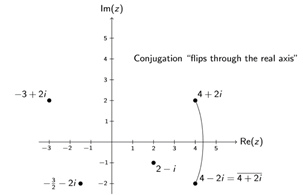
\includegraphics{/home/ryan/gitpage/ryangreenup.github.io/AbstractAlgebraNotes/1551604985277.png}
\caption{}
\end{figure}

And any complex number can be represented also in polar notation:

\begin{align}
z &= a +bi = r \cdot \text{cis}(\theta) \\
\end{align}

Where:

\begin{quote}
\(r = \sqrt{a^2 +b^2} \\
\theta = \text{Atan}(\frac{b}{a})\)
\end{quote}

And the combination is equivalent because:

\begin{align}
\text{cis}(\theta) & = \cos(\theta) + i \cdot \sin(\theta) \\
&= \cos{\theta} + i\cdot \sin{\left ( \text{Asin}\left( \frac{b}{a} \right ) \right )} \\
&=a + bi
\end{align}

Flowing from power series for exponential, cosine and sine functions we
have also:

\[z = a + bi = r \text{cis}(\theta) = e^{i\theta}\]

\hypertarget{header-n965}{%
\subsubsection{Multiplying Complex Numbers}\label{header-n965}}

Polar notation makes it far easier to multiply complex numbers

\begin{quote}
Remember that multiplying a number on the complex plane is
\href{https://www.youtube.com/watch?v=mvmuCPvRoWQ}{really a
transformative process} involving scaling and rotating the plane from
the point 1 (the multiplicative identity) top the point of the
multiplier.

Hence it stands to reason that the distance from the origin of the new
point will be larger by a factor of the scaling and the rotation on the
plane will simply be added.
\end{quote}

For:

\[u = r\cdot \text{cis}(\theta) \enspace \text{and} \enspace v = s \cdot \text{cis}(\phi) \\
\ \\
u\cdot v = rs \cdot \text{cis}(\phi + \theta)\]

\hypertarget{header-n974}{%
\subsubsection{Power of Complex Numbers (De Moivre's
Theorem)}\label{header-n974}}

If follows algebraically that raising complex numbers to the power of
some \(n\):

\begin{align}
z &= r \cdot \text{cis}(\theta) \\
  &\implies z^n = r^n \cdot \text{cis}(n\cdot \theta) \enspace : \enspace n \in \mathbb{Z^*}
\end{align}

\begin{quote}
Recall that \(\mathbb{Z^*}\) is the set of non-negative integers \{0, 1,
2, 3, 4 ...\}.

\begin{quote}
This is an important distinction from \(\mathbb{N}\) because although
many texts provide \(0 \notin \mathbb{N}\) using the reasoning that the
naturals are the various possible sums of 1, many authors provide
\(0 \in \mathbb{N}\) where it is convenient, so try not to use
\(\mathbb{N}\) because it can be ambiguous
\end{quote}
\end{quote}

\hypertarget{header-n983}{%
\subsubsection{Roots of Complex Numbers}\label{header-n983}}

Multiple Complex Numbers, when raised to a power, may equal the same end
result, hence solutions for \(z\) given \(z^n\) are:

\[z^{1/n} = r ^{1/n} \cdot \text{cis}\left( \frac{\theta + 2k\pi}{n} \right ), \quad \text{for} k = 1,2,3, \dots (n-1)\]

There are always \(n\) roots.

\hypertarget{header-n988}{%
\section{Endnotes}\label{header-n988}}

Notes on Polynomials and the Fundamental Theorem of Arithmetic are
contained in the PDF file.

I don't have any notes whatsoever on anything thereafter.

\hypertarget{header-n994}{%
\section{collapsible markdown?}\label{header-n994}}

\hypertarget{header-n996}{%
\section{Notes on Markdown}\label{header-n996}}

\begin{itemize}
\item
  Small MathBlocks on iPhone

  \begin{itemize}
  \item
    If numbered equations are used, they will render extremely small on
    an iPhone, is the trade off worth it?

    \begin{itemize}
    \item
      It's relatively easy to enable and disable numbered mathblocks in
      \emph{Typora} on the fly through the preferences Ctrl + , on mac ⌘
      + , 
    \end{itemize}
  \end{itemize}
\end{itemize}

\href{}{Topic 1}

\end{document}
